\chapter{Programación lineal}
\section{Objetivo de la programación lineal e interpretación en $\IR^3$}
El objetivo de la programación lineal es resolver el problema de
minimizar o maximizar una función $f:\IR^n\rightarrow\IR$
restringida a un dominio $D\subset\IR^n$ de manera que tanto $f$ como
$D$ cumplan ciertas condiciones.

\ifthenelse{\equal{\PDFMODE}{1}}{
  \begin{figure}[h]
    \centering
    \begin{subfigure}[b]{0.3\textwidth}
      \includegraphics[width=\textwidth]{2_INTRO_1.pdf}
      \caption{Una aplicación $f$ lineal}
    \end{subfigure}
    ~
    \begin{subfigure}[b]{0.3\textwidth}
      \includegraphics[width=\textwidth]{2_INTRO_2.pdf}
      \caption{Una $D$ región dada por restricciones}
    \end{subfigure}
    ~
    \begin{subfigure}[b]{0.3\textwidth}
      \includegraphics[width=\textwidth]{2_INTRO_3.pdf}
      \caption{La aplicación lineal $f$ restringida a $D$}
    \end{subfigure}
  \end{figure}
}{
  \begin{figure}
    \includegraphics[width=\textwidth]{2_INTRO_1.pdf}
    \caption{Una aplicación $f$ lineal}
  \end{figure}

  \begin{figure}
    \includegraphics[width=\textwidth]{2_INTRO_2.pdf}
    \caption{Una $D$ región dada por restricciones}
  \end{figure}

  \begin{figure}
    \includegraphics[width=\textwidth]{2_INTRO_3.pdf}
    \caption{La aplicación lineal $f$ restringida a $D$}
  \end{figure}
}
A la función $f:\IR^n\rightarrow\IR$ se le pide que sea lineal y a $D$
que sea un conjunto definido por desigualdades lineales.

\section{Definiciones}

\begin{definicion}[Problema de programación lineal]
  Un problema de programación lineal (PPL) es un problema matemático que se puede expresar de la siguiente forma: \\
  Hallar el máximo / mínimo de una función lineal, $f(x)=c_1x_1+c_2+x_2+...+c_nx_n$ sujeto a una serie de restricciones que podemos expresar como:
  \begin{equation*}
    \left\lbrace
      \begin{array}{l}
        a_{11}x_1+a_{12}x_2+...+a_{1n}x_n \leq b_1 \\
        ... \\
        a_{s1}x_1+a_{s2}x_2+...+a_{sn}x_n \leq b_s \\
        ... \\
        a_{t1}x_1+a_{t2}x_2+...+a_{tn}x_n \leq b_t \\
        ... \\
        a_{t+1,1}x_1+a_{t+1,2}x_2+...+a_{t+1,n}x_n = b_{t+1} \\
        ... \\
        a_{m1}x_1+a_{m2}x_2+...+a_{mn}x_n = b_{m}
      \end{array}
    \right.
  \end{equation*}
  Donde $x_i, a_{ij}, b_j \in \mathbb{R}$ para todo $1\leq i \leq n$, $1 \leq j \leq m$. \\
  Nótese que lo que expresa entre llaves corresponde a una restricción que puede ser hecha a través de desigualdades o igualdades.
\end{definicion}

Se supone sin pérdida de generalidad que $b_j\ge0$ con $1\le j\le m$ (de no ser así bastaría con multiplicar por $(-1)$).

\begin{definicion}[Formato Estándar de un P.P.L]
  Un P.P.L está en formato estándar si está expresado de la siguiente forma:
  $$
  \begin{array}{c}
    \min/\max \quad c_1x_1+c_2x_2+\dots+c_nx_n \vspace*{0.3cm}\\
    \text{s.a} \; \left\{
    \begin{array}{ccccccccc}
      a_{11}  x_1& + & a_{12}x_2 &+&\cdots&+ & a_{1n} x_n&= & b_1\\
      a_{21}  x_1& + & a_{22}x_2 &+&\cdots&+ & a_{2n} x_n&= & b_2\\
      \vdots&  & \vdots & & & &\vdots &  & \vdots\\
      a_{m1}  x_1& + & a_{m2}x_2 &+&\cdots&+ & a_{mn} x_n&= & b_m\\
    \end{array}
    \right.
  \end{array}
  $$
    
  con $x_i\ge0$ para $1\le i\le n$ y $b_j\ge0$ para $1\le j\le m$.
\end{definicion}


\subsection{Forma matricial y conversión de formato}

El problema de programación lineal puede expresarse de forma matricial como:
$$\begin{formulacion}{\min/\max}{1}{c^tx}
  Ax & = & b\\
  x & \ge & 0
\end{formulacion}$$

con $b\ge0$. De esta forma se tiene que

\begin{itemize}
  \item $c^tx:=\text{función objetivo}$
  \item $x:=\text{variables de decisión}$
  \item $c:=\text{vector de costos}$
  \item $A:=\text{matriz de coeficientes tecnológicos}$
  \item $c^tx:=\text{vector de recursos}$
\end{itemize}

Dado cualquier P.P.L siempre es posible transformarlo en otro P.P.L
equivalente (con las mismas soluciones) en formato estándar.

\subsubsection{Conversión de variables}

\begin{itemize}
  \item En el caso de que una variable sea $x_i\le0$ se transforma creando una nueva variable $x_i^*=-x_i\ge0$. De esta forma siempre que aparezca $x_i$ la sustituiremos por $-x_i^*$.
  
  \item En el caso de que $x_i$ sea libre se expresa como la diferencia de dos nuevas variables la correspondiente a la parte positiva y a la negativa ($x_i^+$ y $x_i^-$ respectivamente) quedando $x_i=x_i^+-x_i^-$ con $x_i^+,x_i^-\ge0$. Como ocurría en el caso anterior, se sustituye la variable en cuestión por $x_i^+-x_i^-$.
\end{itemize}

\subsubsection{Conversión de restricciones}

\begin{itemize}
  \item Si nos encontramos con una restricción del tipo $\ge$,
  $$a_{j1}x_1+a_{j2}x_2+\cdots+a_{jn}x_n\le b_j,$$
  
  se añade una nueva variable $s_j\ge0$ y se suma al primer miembro de la desigualdad de modo que esta quedaría de la forma
  $$a_{j1}x_1+a_{j2}x_2+\cdots+a_{jn}x_n + s_j= b_j.$$
  
  \item Si nos encontramos con una restricción del tipo $\le$
  $$a_{j1}x_1+a_{j2}x_2+\cdots+a_{jn}x_n\le b_j,$$
  
  vuelve a introducirse una variable $s_j\ge0$, pero en este caso se resta al primer miembro de la desigualdad de modo que la esta quedaría de la forma
  $$a_{j1}x_1+a_{j2}x_2+\cdots+a_{jn}x_n - s_j= b_j.$$
\end{itemize}

A las variables $s_j$ se las denominan variables de holgura.

\subsubsection{Conversión del vector de recursos}
Si $b_j<0$ entonces multiplicamos por $(-1)$ la restricción $j$-ésima o lo que es equivalente, la fila $j$-ésima de la matriz $A$ y del vector de recursos $b$.

\begin{ejemplo}
  Pasar a formato estándar el siguiente problema
  $$\begin{formulacion}{\min}{4}{2x_1+3x_2+9x_3-x_4}
    x_1 &-x_2& + 4x_3 & &\le & 17\\
    x_1 &+x_2& + x_3 & +x_4 &= & 100\\
    3x_1 &+2x_2& + 9x_3 & -8x_4 &\ge & 5\\
    -x_1 &+x_2& - x_3 & -4x_4 &\ge & -3\\
  \end{formulacion}$$
  
  con $x_1\le0$, $x_2\ge0$, $x_3$ libre y $x_4\ge0$.
\end{ejemplo}

Esto es, los problemas
$$\begin{formulacion}{\max}{2}{c_1x_1+c_2x_2}
  a_{11}x_1& +a_{12}x_2 & \le& b_1\\
  a_{21}x_1& +a_{22}x_2 & \le& b_2\\
  \multicolumn{2}{r}{x_1,x_2}&\ge & 0
\end{formulacion} \equiv \; 
\begin{formulacion}{\max}{3}{c_1x_1+c_2x_2+0s_1+0s_2}
  a_{11}x_1& +a_{12}x_2 &+s_1 & = & b_1\\
  a_{21}x_1& +a_{22}x_2 &+s_2 & = & b_2\\
  \multicolumn{3}{r}{x_1,x_2,s_1,s_2}&\ge & 0
\end{formulacion}$$

son equivalentes, siendo sus soluciones $x=(x_1,x_2)$ y $x'=(x_1,x_2,s_1,s_2)$ respectivamente.

Para empezar, el dominio que define el problema ({\sc II}) coincide con el que define el problema ({\sc I}) cuando se tienen en cuenta sólo las variables $x_1$, $x_2$. Es decir, cuando se re... en ese subespacio. Además, las variables $s_1$ y $s_2$ no están presentes en la función objetivo, por lo que los valores de la f.o. en ambos problemas debe coincidir.

Sea $x$ la solución factible de $[P_1]$. Entonces $x=(x_1,x_2)$ verifica que 
$$
\begin{array}{c}
    a_{11}x_1 +a_{12}x_2 \le b_1\\
    a_{21}x_1 +a_{22}x_2 \le b_2\\
    x_1,x_2\ge 0
\end{array}
$$

por lo que tomando
$$
\begin{array}{c}
  s_1=b_1-a_{11}x_1 -a_{12}x_2 \le 0\\
  s_2=b_2-a_{21}x_1 -a_{22}x_2 \le 0\\
\end{array}
$$

entonces el vector $x'=(x_1,x_2,s_1,s_2)$ es solución de $[P_2]$.

De la misma forma se prueba que $[P_2]$ tiene las mismas soluciones que $[P_1]$.

\begin{definicion}[Solución factible]
  Dado un P.P.L $[P]$
  $$[P] \quad
  \begin{formulacion}{\min}{2}{c'x}
    Ax&=& b\\	
    x&\ge&0
  \end{formulacion}$$
  
  se dice que $x_0$ es solución factible para $[P]$ si cumple que $Ax_0=b$ y $x_0\ge0$.
\end{definicion}


\begin{definicion}[Región factible]
  El conjunto formado por todos los puntos factibles se denomina región factible y se denotará por $R$.
\end{definicion}

\begin{definicion}[Solución óptima]
  Se dice que $x_0\in \IR^n$ es solución óptima de $[P]$ si es factible y cumple que $c^tx\ge c^tx_0$ para todo $x\in R$.
\end{definicion}

\newpage
\subsection{Resolución gráfica de un P.P.L.}

\begin{ejemplo}\label{ej2.2}
  Una fábrica de dos tipos de juguetes: \textbf{soldados} y \textbf{trenes}. Cada soldado se vende por 27 u.m. y se gastan 10 u.m. en materia prima para su fabricación. Cada tren se vende por 21 u.m. y se necesitan para su fabricación 9 u.m. de materia prima. Cada tren eleva el coste de producción en 10 u.m. y cada soldado en 14 u.m. Ambos juguetes necesitan un ensamblado y un acabado, siendo necesarias 1 h. para el acabado y 1 h para el ensamblado de cada tren y 1 h. de ensamblado y 2h. de acabado para cada soldado.\vspace*{0.3cm}
  
  Se disponen de 100 h. de acabados y 80 h. de ensamblado semanales. Además, en esta franja de tiempo sólo pueden venderse 40 soldados como máximo.\vspace*{0.3cm}
  
  ¿Cuántos soldados y trenes debemos producir por semana para obtener el máximo beneficio?
\end{ejemplo}

\ifthenelse{\equal{\PDFMODE}{1}}{
  \begin{figure}[h]
    \centering
    \begin{subfigure}[b]{0.3\textwidth}
      \includegraphics[width=\textwidth]{2_RGRAFICA_1.pdf}
      \caption{Todas las restricciones}
    \end{subfigure}
    ~
    \begin{subfigure}[b]{0.3\textwidth}
      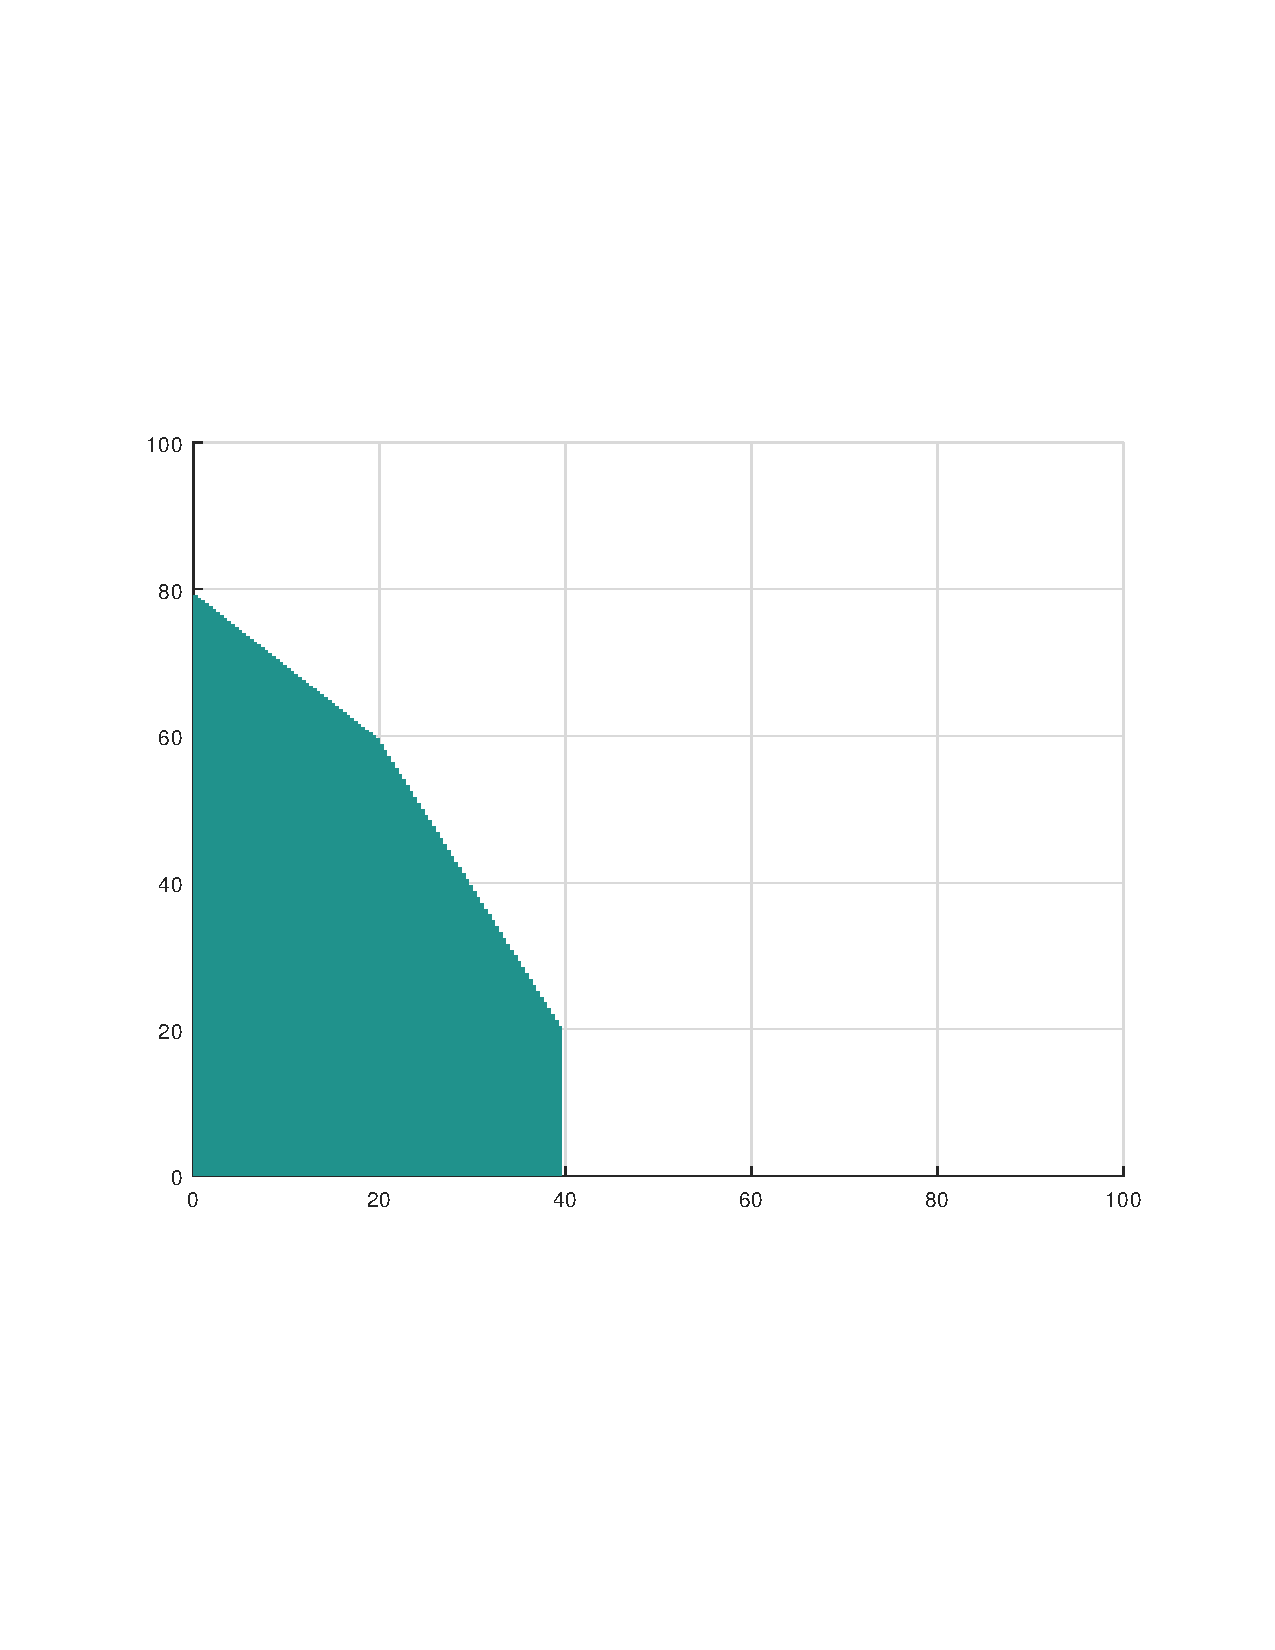
\includegraphics[width=\textwidth]{2_RGRAFICA_2.pdf}
      \caption{Intersección restricciones}
    \end{subfigure}
    ~
    \begin{subfigure}[b]{0.3\textwidth}
      \includegraphics[width=\textwidth]{2_RGRAFICA_3.pdf}
      \caption{Dirección soluciones}
    \end{subfigure}
  \end{figure}
}{
  \begin{figure}
    \includegraphics[width=\textwidth]{2_RGRAFICA_1.pdf}
    \caption{Todas las restricciones}
  \end{figure}

  \begin{figure}
    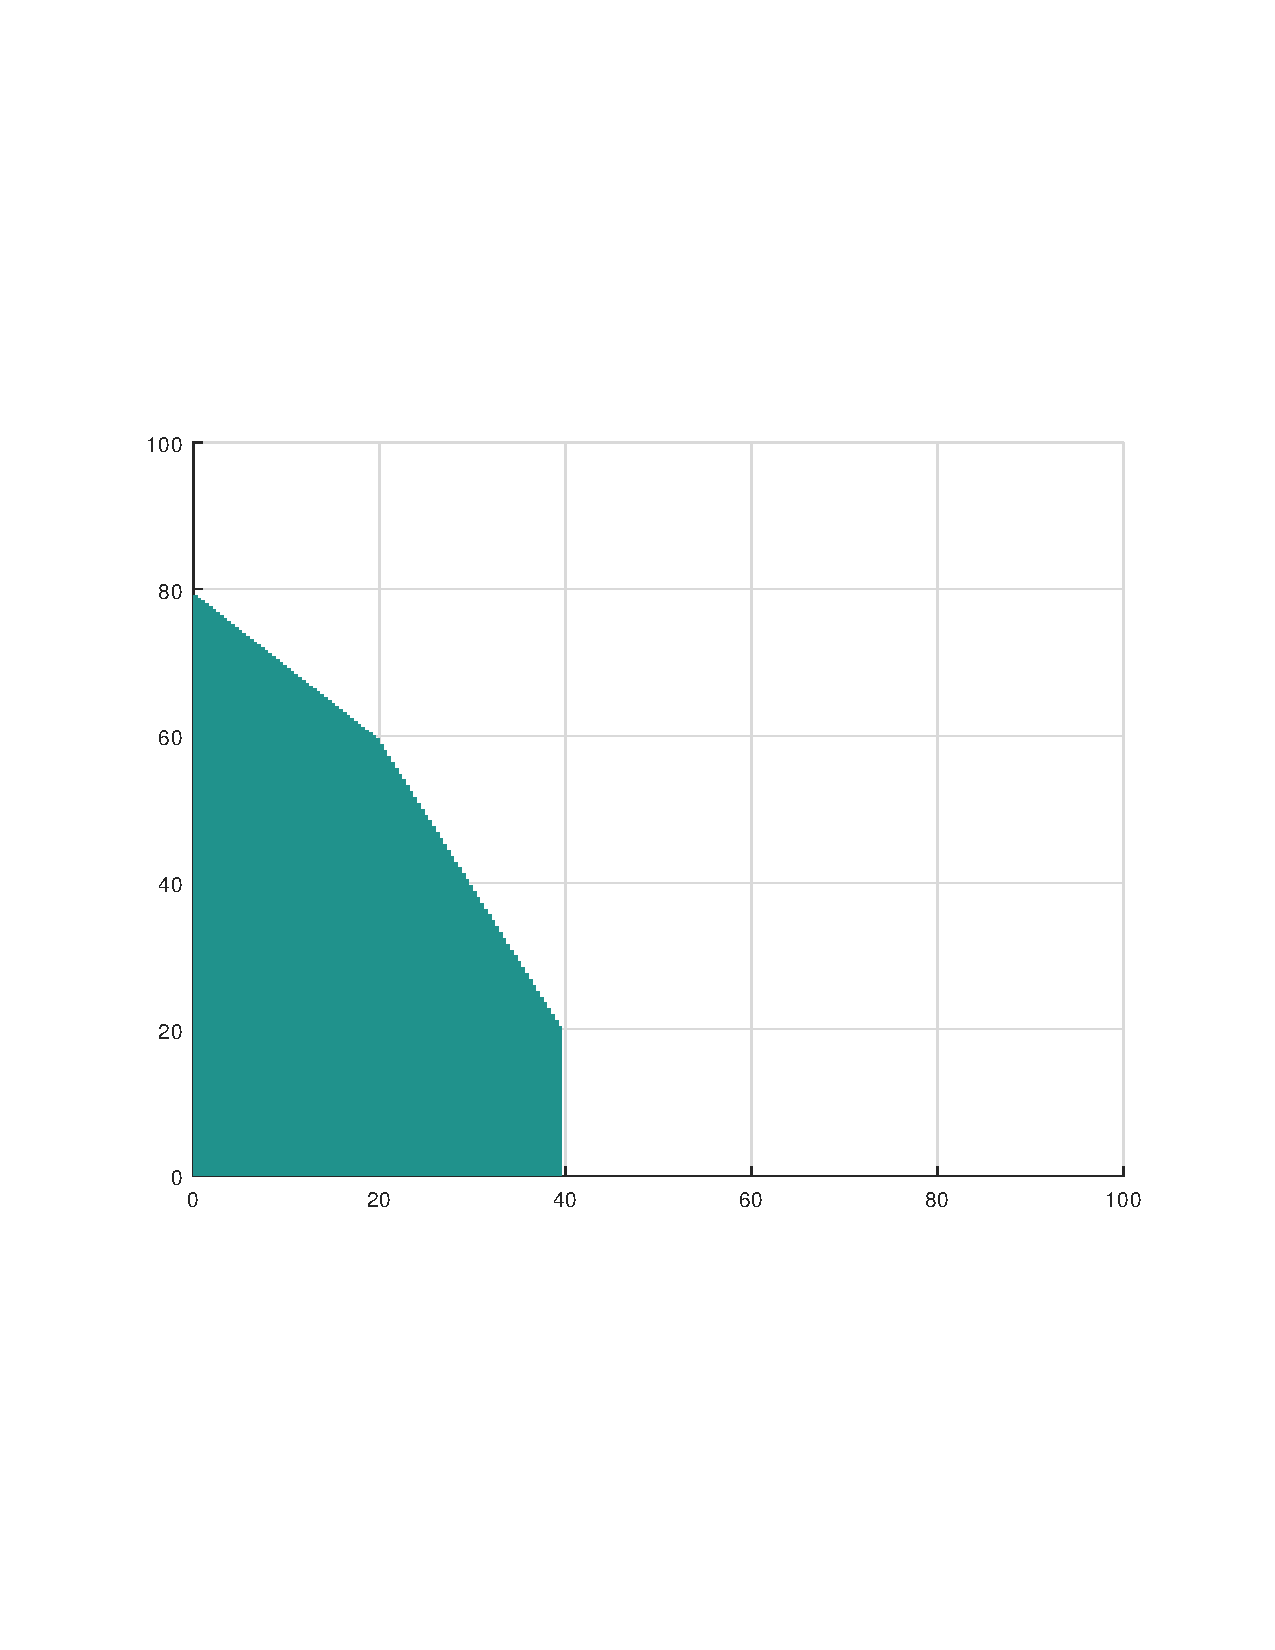
\includegraphics[width=\textwidth]{2_RGRAFICA_2.pdf}
    \caption{Intersección restricciones}
  \end{figure}

  \begin{figure}
    \includegraphics[width=\textwidth]{2_RGRAFICA_3.pdf}
    \caption{Dirección soluciones}
  \end{figure}
}

\begin{definicion}[Restricción activa]
  Dado un P.P.L $[P]$ se dice que una restricción está activa en $x_0$ si se cumple por igualdad en $x_0$.
\end{definicion}

En el ejemplo \ref{ej2.2}, la restricción $s+t\le80$ está activa en $x_0=(20,60)$ pues $20+60=80$.

\subsection{Tipos de P.P.L. según las soluciones}

Podemos clasificar todos los P.P.L:

\begin{itemize}
  \item Si $R=\emptyset$ entonces diremos que el problema es infactible, no tiene solución.
  
  \item Si $R\neq\emptyset$ entonces el problema puede:
  \begin{enumerate}
    \item Tener solución óptima, única o múltiple (infinitas soluciones).
    \item Ser no acotado, es decir, se encuentran soluciones que minimizan(maximizan) la función objetivo tanto como se quiere.
  \end{enumerate}
\end{itemize}

A continuación se ilustran los diferentes casos de forma gráfica.

% TODO: Gráficos tipos de soluciones
\LARGE{METE GRÁFICOS}
\normalsize

\section{Geometría de conjuntos convexos}

\begin{definicion}[Conjunto convexo]
  Un conjunto $S\subseteq \IR^n$ se dice convexo si dados $x,y\in S$ se tiene que $\lambda x + (1-\lambda)y\in S$ para cualquier $\lambda\in (0,1)$.
\end{definicion}

\begin{proposicion}\label{prop2.1}
  La intersección finita de conjuntos convexos es convexa.	
\end{proposicion}

\begin{proof}
  Sean $S_1,S_2,\dots,S_k$ conjuntos convexos de $\IR^n$ con $k\in\IN$ y denotemos
  $$ S = \displaystyle\bigcap_{i=1}^k S_i.$$
  
  Dados $x,y \in S$ entonces $x,y\in S_i$ para todo $i=1,\dots,k$. Como cada $S_i$ es convexo, dado $\lambda\in(0,1)$ se tiene que $\lambda x +(1-\lambda) y \in S_i $ para cada $i=1,\dots,k$ y por tanto $\lambda x +(1-\lambda) y \in S$.
  
  Luego $S$ es convexo.
  
\end{proof}

\begin{definicion}
  Sea $a\in \IR^n$ con $a\neq0$ y $b\in \IR^n$, se define como:
  
  \begin{enumerate}
    \item Hiperplano de $\IR^n$ al conjunto $H=\{x\in\IR^n:a^tx=b\}$.
    \item Semiespacio cerrado positivo a  $H^+=\{x\in\IR^n:a^tx\ge b\}$.
    \item Semiespacio cerrado negativo a $H^-=\{x\in\IR^n:a^tx\le b\}$.
    
  \end{enumerate}
\end{definicion}

\begin{definicion}
  \label{def2.9}
  Un polítopo es un conjunto definido por un número finito de intersecciones de semiespacios o hiperplanos.
  Si un polítopo es acotado entonces se denomina poliedro.
\end{definicion}

Observemos, que en un P.P.L la región factible es un polítopo.

\begin{proposicion}
  Los polítopos son conjuntos convexos.
\end{proposicion}


\begin{proof}
  Teniendo en cuenta la definición \ref{def2.9} y la proposición \ref{prop2.1} basta con demostrar que los semiespacios e hiperplanos son conjuntos convexos.
  
  Sean $x,y\in H^- = \{x\in\IR^n:a^tx\le b\}$ y $\lambda\in(0,1)$. Entonces $a^tx,a^tx\le b$ y como $\lambda>0$ entonces
  \begin{eqnarray}
    \lambda(a^tx) & \le &\lambda b \label{eqp2.2.1}\\
    (1-\lambda)(a^ty) & \le & (1-\lambda)b. \label{eqp2.2.2}
  \end{eqnarray}
  
  Sumando las ecuaciones (\ref{eqp2.2.1}) y (\ref{eqp2.2.2}) se tiene que
  \begin{eqnarray*}
    a^t[\lambda x+(1-\lambda)y]&=& a^t(\lambda x)+a^t[(1-\lambda)y]\\
                               &= &\lambda (a^tx)+(1-\lambda)(a^ty)\\
                               &\le & \lambda b+(1-\lambda)b = b.
  \end{eqnarray*}
  
  Luego $\lambda x+(1-\lambda)y \in H^-$ y por tanto es convexo. Para los conjuntos $H^+$ y $H$ se demuestra de forma similar.
\end{proof}


\begin{definicion}[Punto extremo]
  Dado $S\subseteq \IR^n$ convexo, se dice que $e\in S$ es un punto extremo de $S$ si no existen $x,y\in S $ de forma que se puede expresar como $e=\lambda x+(1-\lambda)y$ para algún $\lambda\in(0,1)$.
  
  INCLUIR REP GRAFICA
\end{definicion}


\begin{definicion}[Dirección de ilimitación (d.d.i.)]
  Dado $S\subseteq \IR^n$ convexo se dice que $d\in\IR^n$ es dirección de ilimitación de $S$ si dado $\lambda\ge0$ entonces $x_0+\lambda d\in S$ para todo $x_0\in S$.
\end{definicion}

%TODO: Gráficos soldados
\LARGE{METE GRÁFICOS}
\normalsize

\begin{definicion}[Dirección de ilimitación extrema]
  Dado $S\subseteq \IR^n$ convexo se dice que $d\in\IR^n$ es d.d.i. extrema de $S$ si no existen $d_1,d_2\in S$ con $d_1\neq d_2$ tal que $d=\lambda_1d_1+\lambda_2 d_2$ con $\lambda_1,\lambda_2>0$.
\end{definicion}



\begin{proposicion}
  Sea $R$ la región factible de un P.P.L. entonces $d$ es dirección de ilimitación de $R$ si y sólo si $Ad=0$ y $d\ge0$.
\end{proposicion}

\begin{proof}
  \begin{enumerate}
    \item[$\Longrightarrow$] Si $d$ es d.d.i. entonces para todo $x_0\in R=\{x\in\IR: Ax=b\}$ y $\lambda\ge0$ se tiene que $x_0+\lambda d\in R$, es decir
    \begin{eqnarray*}
      A(x_0+\lambda d) & = & b\\
      Ax_0 +\lambda Ad & = & b\\
      b + \lambda Ad & = & b\\
      \lambda Ad & = & 0
    \end{eqnarray*}
    
    Luego $Ad=0$.
    
    \item[$\Longleftarrow$] Si $Ad = 0 $ entonces dados $x_0\in R $ y $\lambda\ge0$ se tiene que 
    $$A(x_0+\lambda d)=Ax_0 +\lambda Ad=b$$
    
    y por tanto que $x_0+\lambda d\in R$.
  \end{enumerate}
\end{proof}


\section{Teorema Fundamental de la P.L.}
\subsection{Hipótesis de partida}

Antes de seguir con los P.P.L. debemos fijar dos hipótesis que son razonables. Dado un problema en formato estándar
$$
\begin{formulacion}{\min}{1}{f(x_1,\dots,x_n)}
  Ax & = & b\\
  x&\ge & 0
\end{formulacion}$$

siendo $A$ una matriz de dimensiones $m\times n$ entonces

\begin{enumerate}
  \item La matriz tenga rango máximo ($rg(A)=m$) ya que, en caso contrario y como veremos más adelante, alguna de las $m$ restricciones sería innecesaria o el problema sería infactible. A esta hipótesis se la conoce como Hipótesis de rango completo.
  \item El número de restricciones será menor que el de incógnitas ($m
  \le n$). Esta hipótesis se deduce de la anterior.
\end{enumerate}
Es importante resaltar que la matriz $A$ es aquella que resulta de
añadir las variables homogéneas, lo que se está pidiendo es que $A$ sea de la forma
$$
\begin{blockarray}{cc}
  \begin{block}{[c]l}
    \hspace*{2.5cm} & \\
    & \\
    & \\
    & _{n\times m}\\
  \end{block}
  A & \\
\end{blockarray}
\begin{blockarray}{cc}
  \begin{block}{[c]l}
    \hspace*{0.3cm}& \\
    & \\
    & \\
    & _{n\times 1}\\
  \end{block}
  x & \\
\end{blockarray}
\begin{array}{c}
  =\\ \\ \\
\end{array}\quad
\begin{blockarray}{cc}
  \begin{block}{[c]l}
    \hspace*{0.3cm}& \\
    & \\
    & \\
    & _{m\times 1}\\
  \end{block}
  b & \\
\end{blockarray}
$$

La hipótesis de rango completo asume que todas las filas de $A$ son
linealmente independientes. de no ser así podría ocurrir dos cosas:

\begin{enumerate}
  \item Si la fila $i$ es linealmente dependiente de la fila $j$ en la
  matriz $A$ pero linealmente independiente en la matriz ampliada
  $[\;A\;|\;b\;]$ entonces el problema es infactible ya  que hay dos
  restricciones contradictorias.
  $$
  \begin{array}{rrrrr}
    2x & + & y & = & 10\\
    4x & + & 2y & = & 10\\
  \end{array}
  $$
  
  El sistema no tiene solución, por lo que el problema es infactible.
  
  \item Si la fila $i$ es linealmente dependiente de  la fila $j$ en
  $[\;A\;|\;b\;]$ entonces estamos ante dos restricciones equivalentes
  y por tanto podemos eliminar una de ellas.
  
\end{enumerate}

De aquí, se deduce que $m$ no puede ser mayor que $n$ pues si fuese
$n<m$ entonces el rango máximo de $A$ sería $n$ y eso significaría que
existen filas de $A$ linealmente dependientes dandose así alguno de
los casos anteriores. Por tanto podemos suponer sin ningún problema
que $m\le n$.

Dado un $P.P.L.$ en formato estándar
$$
\begin{formulacion}{\max}{1}{c^tx}
  Ax & = & b\\
  x & \ge & 0
\end{formulacion}
$$

siendo 
$$
\begin{blockarray}{cc}
  A & \\
  \begin{block}{[c]l}
    \multirow{4}{*}{$a_1\;\cdots\; a_m\;\cdots\; a_n$} & \\
    & \\
    & \\
    & _{n\times m}\\
  \end{block}
\end{blockarray}
\begin{blockarray}{cc}
  x & \\
  \begin{block}{[c]l}
    \hspace*{0.3cm}& \\
    & \\
    & \\
    & _{n\times 1}\\
  \end{block}
\end{blockarray}
\begin{array}{c}
  = \\
\end{array}\quad
\begin{blockarray}{cc}
  b & \\
  \begin{block}{[c]l}
    \hspace*{0.3cm}& \\
    & \\
    & \\
    & _{m\times 1}\\
  \end{block}
\end{blockarray}
$$

Como $rg(A)=rg(A|b)=m<n$ entonces el sistema es compatible indeterminado (existen infinitas soluciones).

\begin{nota}
  El caso $m=n$ es trivial ya que implica que hay solución única y por tanto esa debe ser la óptima.
\end{nota} 

Las columnas de $A$ deben ser linealmente dependientes y por tanto existe $m$ columnas linealmente independientes. Formemos pues una nueva submatriz $B$ con $m$ columnas de $A$ linealmente independientes. Sin pérdida de generalidad, podemos suponer que tomamos las $m$ primeras. Entonces el sistema se descompone como sigue:
\begin{equation}
  \left[
    \begin{array}{cc}
      \scalebox{1.5}{B} & \scalebox{1.5}{N}
    \end{array}
  \right]
  \left[
    \begin{array}{c}
      x_B \\ x_N
    \end{array}\right]=
  \left[
    \begin{array}{c}
      \multirow{2}{*}{b} \\
      \\
    \end{array}\right].\label{desc2.1}
\end{equation}

El subsistema formado por $Bx_B=b$ tiene solución única pues $B$ es
cuadrada con $|B|\neq0$, lo que significa que si tomamos $x_N=0$
obtenemos una solución para el sistema original
$$Bx_B+N\cdot0=b.$$

\begin{definicion}[Solución básica]
  Dado un P.P.L. en formato estándar, a la solución única $x_B$
  procedente de la descomposición (\ref{desc2.1}) se la denomina
  solución básica, y existen como máximo $$
  \left(
    \begin{array}{c}
      n \\ m
    \end{array}
  \right)\;\text{posibles soluciones.}$$
\end{definicion}

\begin{ejemplo}
	Consideremos el problema 
	$$
        \begin{formulacion}{\max}{3}{3x_1+2x_2}
          1x_1 &+4x_2 & -s_1 &=& 17\\
          0 x_1 & + 7x_2 &+ s_2 &=& 10 \\
          \multicolumn{3}{r}{x_1,x_2,s_1,s_2}&\ge&0
        \end{formulacion}
        $$
	
	Entonces se tiene que
	$$
        \left(
          \begin{array}{rrrr}
            1 & 4 & -1 & 0\\
            0 & 7 & 0  & 1
          \end{array}\right)
	\left(
          \begin{array}{r}
            x_1 \\ x_2\\ s_1\\ s_2
          \end{array}\right)
	=
	\left(
          \begin{array}{r}
            17\\ 10
          \end{array}
        \right),$$
	
	y por tanto que una descomposición del tipo (\ref{desc2.1}) es:
	$$
        B=\left(
          \begin{array}{rr}
            1 & 0\\
            0 &  1
          \end{array}
        \right),\qquad
	x_B=\left(
          \begin{array}{r}
            x_1 \\ s_2
          \end{array}
        \right).$$
	
	Quedando que $Bx_B=b$ y por tanto $x_B=\left(\begin{array}{r}17\\10\end{array}\right)$. Luego $x^t=(17,0,0,10)$.
\end{ejemplo}

\begin{nota}
  Existen soluciones básicas no factibles, es decir, no toda solución básica sirve, sólo las soluciones básicas factibles.
\end{nota}

\begin{definicion}
  En las mismas condiciones de antes, las variables $x_i$ que se
  corresponden con las columnas de la base $B$ se las denominan
  Variables básicas. \\
  
  Al resto se las denominan variables no básicas (y siempre se igualan a cero).
\end{definicion}

\begin{definicion}
  Dada una solución básica, si alguno de sus componentes básicos es cero entonces se lo denomina Solución básica degenerada.
\end{definicion}

\begin{definicion}[Soluciones básicas adyacentes]
  Dos soluciones básicas se dicen adyacentes si sus bases son iguales excepto en una columna.
\end{definicion}

\begin{nota}
  El siguiente teorema nos da una interpretación geométrica de qué es una solución básica.
\end{nota}

\begin{teorema}
  Sea $A_{m\times n}$ con $rg(A)=m<n$. Sea
  $R=\{x:Ab=b,\;x\ge0\}$. Entonces se tiene que $x_0$ es solución
  básica factible si y sólo si $x_0\in R$ y es punto extremo de $R$.
\end{teorema}

\begin{proof}
  \begin{enumerate}
    \item[$\Longrightarrow$] Si $x_0$ es solución básica factible y por tanto, por ser factible, $x_0\in R$. Veamos por reducción al absurdo que $x_0$ es punto extremo de $R$.
    
    Supongamos pues que $x_0$ no es punto extremo de $R$. Entonces existen $x,y\in R$ con $x\neq y$ y $\lambda\in(0,1)$ tal que $x_0=\lambda x + (1-\lambda)y$.
    
    Al ser $x_0$ solución básica, se puede expresar sin pérdida de generalidad como:
    $$
    x_0=
    \left(
      \begin{array}{c}
        x_{01}\\ \vdots \\x_{0p}\\ 0 \\ \vdots \\ 0
      \end{array}\right) \text{ donde $p\le m$.}$$
    
    Observemos que se está teniendo en cuenta que $x_0$ sea una solución básica degenerada. Además, en el caso de que $x_0=\overline{0}$, este punto es punto extremo de $R$ pues:
    $$x_0=\overline{0}=
    \left(
      \begin{array}{c}
        0\\\vdots\\0
      \end{array}\right)=
    \lambda
    \left(
      \begin{array}{c}
        x_1\\\vdots\\ x_n
      \end{array}\right)
    +(1-\lambda)
    \left(
      \begin{array}{c}
        y_1\\\vdots\\ y_n
      \end{array}
    \right),$$
		
    pero $\lambda x_i + (1-\lambda)y_i=0$ se verifica si y sólo si $x_i=y_i=0$. Luego $\overline{0}$ es un punto extremo.
		
    Consideremos entonces que $x_{0i}>0$ para $1\le i\le p$. Como $x_0$ es solución básica, se verifica que las primeras $p$ variables o columnas de $A$ son linealmente independientes.
		
    Además, $x$ e $y$ deben tener la siguiente expresión por el mismo argumento de antes:
    $$x=\left(
      \begin{array}{c}
        x_{1}\\ \vdots \\x_{p}\\ 0 \\ \vdots \\ 0
      \end{array}\right)\; \text{ e }\;
    y=\left(
      \begin{array}{c}
        y_{1}\\ \vdots \\y_{p}\\ 0 \\ \vdots \\ 0
      \end{array}
    \right).$$
    
    Como $x,y\in R$ entonces $Ax=Ay=b$ y por tanto $A(x-y)=0$. Esto es
    $$\left(
      \begin{array}{ccccc}
        & & & &\\
        a_1 &\cdots & a_p &\cdots & a_n\\
        & & & &
      \end{array}
    \right)
    \left(
      \begin{array}{c}
        x_1-y_1\\
        \vdots\\
        x_p-y_p\\
        0\\
        \vdots\\
        0
      \end{array}
    \right)
    =
    \left(
      \begin{array}{c}
        0\\
        \vdots\\
        0
      \end{array}
    \right),$$
		
    esto es $a_1(x_1-y_1)+a_2(x_2-y_2)+\cdots+a_p(x_p-y_p)=\overline{0}$.
    
    Como cada $A_i$ son linealmente independientes entonces $x_i-y_i=0$ para $1\le i \le p$. Es decir $x=y$ llegando así a una contradicción. Luego $x_0$ es un punto extremo de $R$.
    
    \item[$\Longleftarrow$] Sea $x_0\in R$ con $x_0$ punto extremo de $R$. Como $x_0\in R$ entonces $Ax_0=b$ y $x_0\ge0$. Veamos que $x_0$ es solución básica. En primer lugar, escribiremos
    $$x_0=\left(
      \begin{array}{c}
        x_{01}\\ \vdots \\x_{0p}\\ 0 \\ \vdots \\ 0
      \end{array}\right) \text{ donde $p\le m$.}$$
		
    Podemos suponer que $p\le m$ sin problemas, pues en el caso de que $m<p<n$ se cumple que $a_1,a_2,\dots,a_p$ son columnas de $A$ linealmente dependientes puesto que $rg(A)=m$ por lo que existen unos escalares no todos nulos tales que
    $$\lambda_1 a_1+\lambda_2 a_2+\cdots+\lambda_p a_p=0.$$
		
    Tomemos $\lambda=(\lambda_1,\dots,\lambda_m,\dots,\lambda_p,\dots,\lambda_n)$, entonces existe $\epsilon>0$ suficientemente pequeño tal que
    $$\left\{
      \begin{array}{l}
        x_0^+=x_0+\epsilon\lambda\in R\\
        x_0^-=x_0-\epsilon\lambda\in R\\
      \end{array}
    \right.$$
		
    y por construcción $x_0=\frac{1}{2}x_0^++\frac{1}{2}x_0^-$ con $x_0^+\neq x_0^-$, por lo que $x_0$ no sería punto extremo de $R$.
		
    Supongamos entonces que $p\le m$. Se tiene que si $a_1,a_2,\dots,a_p$ son  columnas linealmente independientes de $A$ entonces $x_0$ sería solución básica. 
		
    Observemos que esto es cierto ya que en el caso de que $a_1,a_2,\dots,a_p$ fuesen linealmente dependientes, por el mismo razonamiento de antes existirían $x_0^+,x_0^-\in R$ con $x_0^+\neq x_0^-$ tal que $x_0=\frac{1}{2}x_0^++\frac{1}{2}x_0^-$ contradiciendo de esta forma que $x_0$ sea punto extremo.
		
    Por tanto $a_1,\dots,a_p$ son linealmente independientes y por tanto $x_0$ es solución básica factible.
  \end{enumerate}
\end{proof}

¿Qué ocurre si $x_0$ proviene de columnas linealmente dependientes donde hay un vector linealmente independiente?
$$
\begin{array}{cccc|ccc}
  \begin{array}{|c|}
    \hline\\\\\\\hline
  \end{array} &
\begin{array}{|c|}\hline\\\\\\\hline\end{array}&
\cdots &
\begin{array}{|c|}\hline\\\\\\\hline\end{array}&
\begin{array}{|c|}\hline\\\\\\\hline\end{array}&
\cdots &
\begin{array}{|c|}\hline\\\\\\\hline\end{array}\\
a_1 & a_2 & & a_m & a_{m+1} & & a_n
\end{array}$$

Supongamos que $a_{m+1}=a_{m+2}=\cdots=a_n$.

\begin{ejemplo}\label{ej2:4}
$$\begin{formulacion}{\min/\max}{5}{c^tx}
x_1 & +x_2 & +x_3 & +x_4 & &= & 1\\
2x_1 & +2x_2 & +2x_3 &  &+x_5 &= & 2\\
\multicolumn{7}{r}{x_i\ge0\quad 1\le i\le 5}
\end{formulacion}$$

$$\begin{simplex}{5}{}
{x_1 & x_2 & x_3 & x_4 & x_5 & b}
{& & 1 & 1 & 1 & 1 & 0 & 1\\
 & & 2 & 2 & 2 & 0 & 1 & 2\\}
       &   &   &   &   &  \\
\end{simplex}$$
\end{ejemplo}

\begin{solucion}
Sea $x_0=\left(\begin{array}{c}
1\\1\\1\\1
\end{array}\right)\in R$, como todas las componentes son positivas veamos si las columnas correspondientes, $a_1$, $a_2$, $a_3$, $a_4$ son linealmente independientes:
$$
\lambda_1a_1+\lambda_2a_2+\lambda_3a_3+\lambda_4a_4= 0
$$
$$
-1\left(
\begin{array}{c}1\\0\\0\end{array}
\right)
-2\left(
\begin{array}{c}0\\1\\0\end{array}
\right)
-3\left(
\begin{array}{c}0\\0\\1\end{array}
\right)
+1\left(
\begin{array}{c}2\\3\\4\end{array}
\right)
 =  0.$$

Sea $\lambda=\left(
\begin{array}{r}
-1\\-2\\-3\\1
\end{array}
\right)$ y $x_0^+=\left(\begin{array}{c}
1\\1\\1\\1
\end{array}\right)+\epsilon\left(
\begin{array}{r}
-1\\-2\\-3\\1
\end{array}
\right)$ con $\epsilon\ge0$. 

Para que $x_0^+\in R$ ha de cumplirse $\left\{\begin{array}{r}
Ax_0^+=0\\x_0^+\ge0
\end{array}\right.$. En primer lugar tenemos que
$$ax_0^+=A(x_0+\epsilon\lambda)=Ax_0+\epsilon\underbrace{A\lambda}_{\text{$=0$}}=Ax_0=b.$$

En segundo lugar, para que se cumpla $x_0^+\ge0$, podemos calcular el mínimo $\epsilon\ge0$ de manera que se anule sólo una componente de $x_0^+$.
$$x_0^+=\left(\begin{array}{l}
1-\epsilon\\
1-2\epsilon\\
1-3\epsilon\\
1+\epsilon
\end{array}\right)\ge0\text{, es decir }
\begin{array}{rcl}
1-\epsilon=0 &\Longleftrightarrow & \epsilon=1\\
1-2\epsilon=0 &\Longleftrightarrow & \epsilon=1/2\\
1-3\epsilon=0 &\Longleftrightarrow & \epsilon=1/3\\
\end{array}$$

por lo que tomando $\epsilon=1/3$ se tiene que
$x_0^+=\left(\begin{array}{c}
2/3\\
1/3\\
0\\
4/3
\end{array}\right)\in R$ y ahora las columnas de las que proviene $x_0^+$ son linealmente independientes: 
\begin{center}
$a_1$, $a_2$ y $a_3$ $\equiv$ $\left(
\begin{array}{c}1\\0\\0\end{array}
\right)$ 
$\left(
\begin{array}{c}0\\1\\0\end{array}
\right)$ y 
$\left(
\begin{array}{c}1\\2\\3\end{array}
\right)$.
\end{center}

\end{solucion}

Antes de proseguir con el Teorema fundamental de la Programacion lineal (teorema \ref{t2:2}) sería conveniente desarrollar un ejemplo donde mostrar el método cosntructivo que demuestra el teorema.

\begin{ejemplo}\label{ej2:5}
$$\begin{formulacion}{}{4}{}
x_1 & &  & +x_4 & = & 2\\
 & x_2 &  & +2x_4 &= & 3\\
  &  & x_3 & +3x_4 &= & 4
\end{formulacion}$$

$$\begin{simplex}{4}{}
{x_1 & x_2 & x_3 & x_4 & b}
{& & 1 & 0 & 0 & 1 & 2\\
 & & 0 & 1 & 0 & 2 & 3\\
 & & 0 & 0 & 1 & 3 & 4\\}
       &   &   &   &   \\
\end{simplex}$$
\end{ejemplo}

\begin{solucion}
Sea $x_0=\left(\begin{array}{c}
1/3\\1/3\\1/3\\0\\0
\end{array}\right)\in R$, se tiene que una solución básica proviene de resolver
$$\frac{1}{3}a_1+\frac{1}{3}a_2+\frac{1}{3}a_3=b,$$

pero $a_1$, $a_2$, $a_3$ son linealmente dependientes, luego existen $\lambda_1=1,\lambda_2=-1,\lambda_3=0\in\IR$ tal que
$$1\left(
	\begin{array}{c}
			1 \\
			2
	\end{array}
\right)-1\left(
	\begin{array}{c}
			1 \\
			2
	\end{array}
\right)+0\left(
	\begin{array}{c}
			1 \\
			2
	\end{array}
\right)=\left(
	\begin{array}{c}
			0 \\
			0
	\end{array}
\right).$$

Sea $\lambda=\left(
\begin{array}{r}
1\\-1\\0\\0\\0
\end{array}
\right)$ entonces $x_0^+=\left(\begin{array}{c}
1/3\\1/3\\1/3\\0\\0
\end{array}\right)+\epsilon\left(
\begin{array}{r}
1\\-1\\0\\0\\0
\end{array}
\right)$ tomando $\epsilon=\dfrac{1}{3}$ se obtiene
$$x_0^+=\left(\begin{array}{c}
2/3\\0\\1/3\\0\\0
\end{array}\right),$$

que es solución factible y proviene de $a_1$ y $a_2$ que son linealmente dependientes por lo que  debemos repetir el proceso.

Sea $\lambda'=\left(
\begin{array}{r}
1\\0\\-1\\0\\0
\end{array}
\right)$ entonces $x_0^{++}=\left(\begin{array}{c}
2/3\\0\\1/3\\0\\0
\end{array}\right)+\epsilon\left(
\begin{array}{r}
1\\0\\-1\\0\\0
\end{array}
\right)$ tomando $\epsilon=\dfrac{1}{3}$,
$$x_0^+=\left(\begin{array}{c}
1\\0\\0\\0\\0
\end{array}\right)\in R,\quad\text{por construcción.}$$

Además se tiene que $a_1$ es linealmente independiente. ¿Pero se puede decir que $x_0^{++}$ es solución básica? Pues sí, en concreto es básica degenerada, porque podemos encontrar $m-1$ vectores de $A$ que sean linealmente independientes y de manera que forman una base junto con $a_1$, sólo tomando que las componentes de dichas columnas sean ceros ya que se tendría que el vector $x_0^{++}$ proviene de una base.
$$\underbrace{\begin{array}{c|cccc}
a_1 & a_1' & a_2 & \cdots & a_{m-1}
\end{array}}_{\text{$m$ columnas l. indep.}}\left(
\begin{array}{c}
1\\0\\0\\0\\0
\end{array}
\right)=\left(
\begin{array}{c}
1\\2
\end{array}\right),$$

luego el $x_0^{++}$ procede de una base y es solución básica.

De la misma forma si el $x_0$ original hubiese tenido dos vectores linealmente independientes bastaria con añadir columnas linealmente independientes hasta completar la base y considerar dichas variables basicas nulas obteniendo asi soluciones basicas degeneradas.
\end{solucion}

\begin{teorema}[Teorema Fundamental de la Programación Lineal]
  \label{t2:2}
  Dado un P.P.L.
  $$
  \begin{formulacion}{\min/\max}{1}{c^t}
    Ax & = & b\\
    x & \ge & 0
  \end{formulacion}$$
  
  \begin{enumerate}
    \item Si existe $x_0$ solución factible de $[P]$ entonces existe
    $x^*$ solución básica factible óptima de $[P]$.

    \item Si existe $x_0$ solución factible óptima de $[P]$ entonces
    existe $x^*$ solución básica factible óptima de $[P]$.
  \end{enumerate}
\end{teorema}


\begin{proof}
  \begin{enumerate}
    \item Sea $x_0$ una solución factible de $[P]$ entonces $x_0$ se puede escribir como
    $$x_0=\left(
      \begin{array}{c}
        x_{01}\\ \vdots \\x_{0p}\\ 0 \\ \vdots \\ 0
      \end{array}\right) \text{ donde $0\le p\le n$.}$$
    
    Para el caso $p=0$ entonces $x_0=\overline0$ es punto extremo y por tanto solución básica(degenerada). Supongamos entonces que $x_{0i}>0$ para $1\le i\le p$ con $1\le p\le n$.
    
    Basta con demostrar que las columnas de a $a_1,a_2,\dots,a_p$ asociadas a esos componentes son linealmente independientes para probar que $x_0$ es solución básica.
    
    Si $a_1,a_2,\dots,a_p$ fuesen linealmente dependientes entonces existen $\lambda_1,\lambda_2,\dots,\lambda_p$ escalares no todos nulos tales que
    $$\lambda_1 a_1+\lambda_2 a_2+\cdots+\lambda_p a_p=0.$$
    
    Definimos $\lambda=(\lambda_1,\dots,\lambda_p,0,\dots,0)\in\IR^n$ y tomamos
    $$x_0^+=x_0+\epsilon\lambda=\left(
      \begin{array}{c}
        x_{01}\\\vdots\\x_{0p}\\0\\\vdots\\0
      \end{array}\right)
    +\epsilon
    \left(
      \begin{array}{c}
        \lambda_{1}\\\vdots\\\lambda_{p}\\0\\\vdots\\0
      \end{array}\right)
    =
    \left(
      \begin{array}{c}
        x_{01}+\epsilon\lambda_1\\
        \vdots\\
        x_{0p}+\epsilon\lambda_p\\
        0\\\vdots\\0
      \end{array}\right).$$
    
    \begin{itemize}
      \item Si existe un $\lambda_1<0$ (o varios) tomamos $$\epsilon=\min\left\{-\dfrac{-x_{oi}}{\lambda_i}: \lambda_i<0\right\}$$
      de esa manera obtendríamos un nuevo vector $x_0^+$ con una componente menos, es decir, ahora tiene $p-1$ componentes mayores estrictas que cero pero aun así $x_0^+\in R$ ya que
      $$Ax_0^+=A(x_0+\epsilon\lambda)=Ax_0+\epsilon\lambda=b.$$
      
      Como $rg(A)=m$ se tendrá que repitiendo el procedimiento $p-m$ veces obtendremos $m$ componentes linealmente independientes, siendo por tanto $x_0$ solución básica.
                                                        
      \item Si todos los $\lambda_i>0$ tomamos el vector $x_0^-=x_0-\epsilon\lambda$ y por el mismo razonamiento anterior, llegaríamos a un vector cn menos componentes estrictamente positivos y sus columnas asociadas linealmente independientes (ver ejemplo \ref{ej2:4}).
    \end{itemize}
    
    \item Si existe una solución factible óptima de $[P]$, llamémosla $x_0\in R$, entonces
    $$x_0=\left(
      \begin{array}{c}
        x_0^1\\\vdots\\x_0^p\\0\\\vdots\\0
      \end{array}
    \right)\text{ con } x_0^i>0 \text{ para }1\le i\le p.$$
    
    \begin{itemize}
      \item Si $a_1,a_2,\dots,a_p$ son columnas de $A$ linealmente independientes entonces $x_0$ es básica.
      \item Si $a_1,a_2\dots,a_p$ son columnas de $A$ linealmente dependientes entonces existen $\lambda_1,\dots,\lambda_p$ escalares no todos nulos tales que $\lambda_1 a_1+\cdots + a_p=0$.
      
      Sea $\lambda^t=(\lambda_1,\dots,\lambda_p,0,\dots,0)\in\IR^n$ y definamos
      $$x_\epsilon^+=x_0+\epsilon\lambda\quad\text{y}\quad x_\epsilon^-=x_0-\epsilon\lambda.$$
      
      Se puede elegir $\epsilon_0>0$ tal que $x_{\epsilon_0}^+,x_{\epsilon_0}^-\in R$. Esto es, $Ax_{\epsilon_0}^+=Ax_{\epsilon_0}^-=b$ y $x_{\epsilon_0}^+,x_{\epsilon_0}^-\le0$. Ahora bien,
      
      \begin{itemize}
        \item Si $c^t\lambda>0$ entonces 
        \begin{eqnarray}
          c^tx_{\epsilon_0}^+=c^tx_0+\epsilon c^t\lambda > c^tx_0\label{ec1tf}\\
          c^tx_{\epsilon_0}^-=c^tx_0-\epsilon c^t\lambda < c^tx_0\label{ec2tf}
        \end{eqnarray}
        
        así pues, las ecuaciones (\ref{ec1tf}) y (\ref{ec2tf}) si $[P]$ es de maximizar o de minimizar respectivamente, contradicen que $x_0$ sea la solución óptima.
        
        \item Si $c^t\lambda<0$ entonces 
        \begin{eqnarray}
          c^tx_{\epsilon_0}^-=c^tx_0-\epsilon c^t\lambda > c^tx_0\label{ec3tf}\\
          c^tx_{\epsilon_0}^+=c^tx_0+\epsilon c^t\lambda < c^tx_0\label{ec4tf}
        \end{eqnarray}
        
        así pues, las ecuaciones (\ref{ec3tf}) y (\ref{ec4tf}) si $[P]$ es de maximizar o de minimizar respectivamente, contradicen que $x_0$ sea la solución óptima.
        
        \item Si $c^t\lambda=0$ entonces $c^tx_0=c^tx_0^+=c^tx_0^-$ por lo que $x_0^+$ y $x_0^-$ son soluciones con el mismo valor de la función objetivo y con una componente menos estrictamente positiva, por lo que repitiendo el proceso de forma iterativa se llegaria a un $x_\epsilon^*=x_0^*\pm\lambda\epsilon$ donde $x_\epsilon^*$ sea básica y $c^tx_\epsilon^*=c^tx_0$.
      \end{itemize} 
    \end{itemize}
  \end{enumerate}
  
\end{proof}


\begin{corolario}
  Si un polítopo es no vacío entonces el conjunto de puntos extremos es no vacío.
\end{corolario}

\begin{corolario}
  Si existe solución óptima finita entonces existe una solución óptima finita que es un punto extremo.
\end{corolario}

\begin{corolario}
  El conjunto de puntos extremos de un polítopo es finito a lo sumo 	
  $$\left(
    \begin{array}{c}
      n\\
      m	
    \end{array}\right).$$
        
\end{corolario}

\begin{ejemplo}
  
  Si consideramos $n=100$ variables y $m=30$ restricciones y cada sistema básico tarda en resolverse 1 milisegundo, se tiene que:
  
  $$\left(
    \begin{array}{c}
      100 \\
      30
    \end{array}\right) = \frac{100!}{70! \cdot 30!} = 29 \cdot 10^{24} = 9195 \ \text{billones de años.}$$
              
\end{ejemplo}

El método SIMPLEX, el cual veremos en el próximo capítulo busca la solución óptima entre las soluciones básicas pero sin calcularlas todas.
